\chapter{Definition of the framework concept\label{cha:chapter4}}

Not only the requirements form the previous chapter \ref{cha:chapter3} but also the analysis and assessment of faulty data in chapter \ref{cha:chapter2} are the basis for the concept design of the framework proposal. This chapter introduces the design of the overall framework and its components as well as its architectural structure.

\section{Overall framework design \label{sec:overalldesign}}

\begin{figure}[htb]
  \centering
  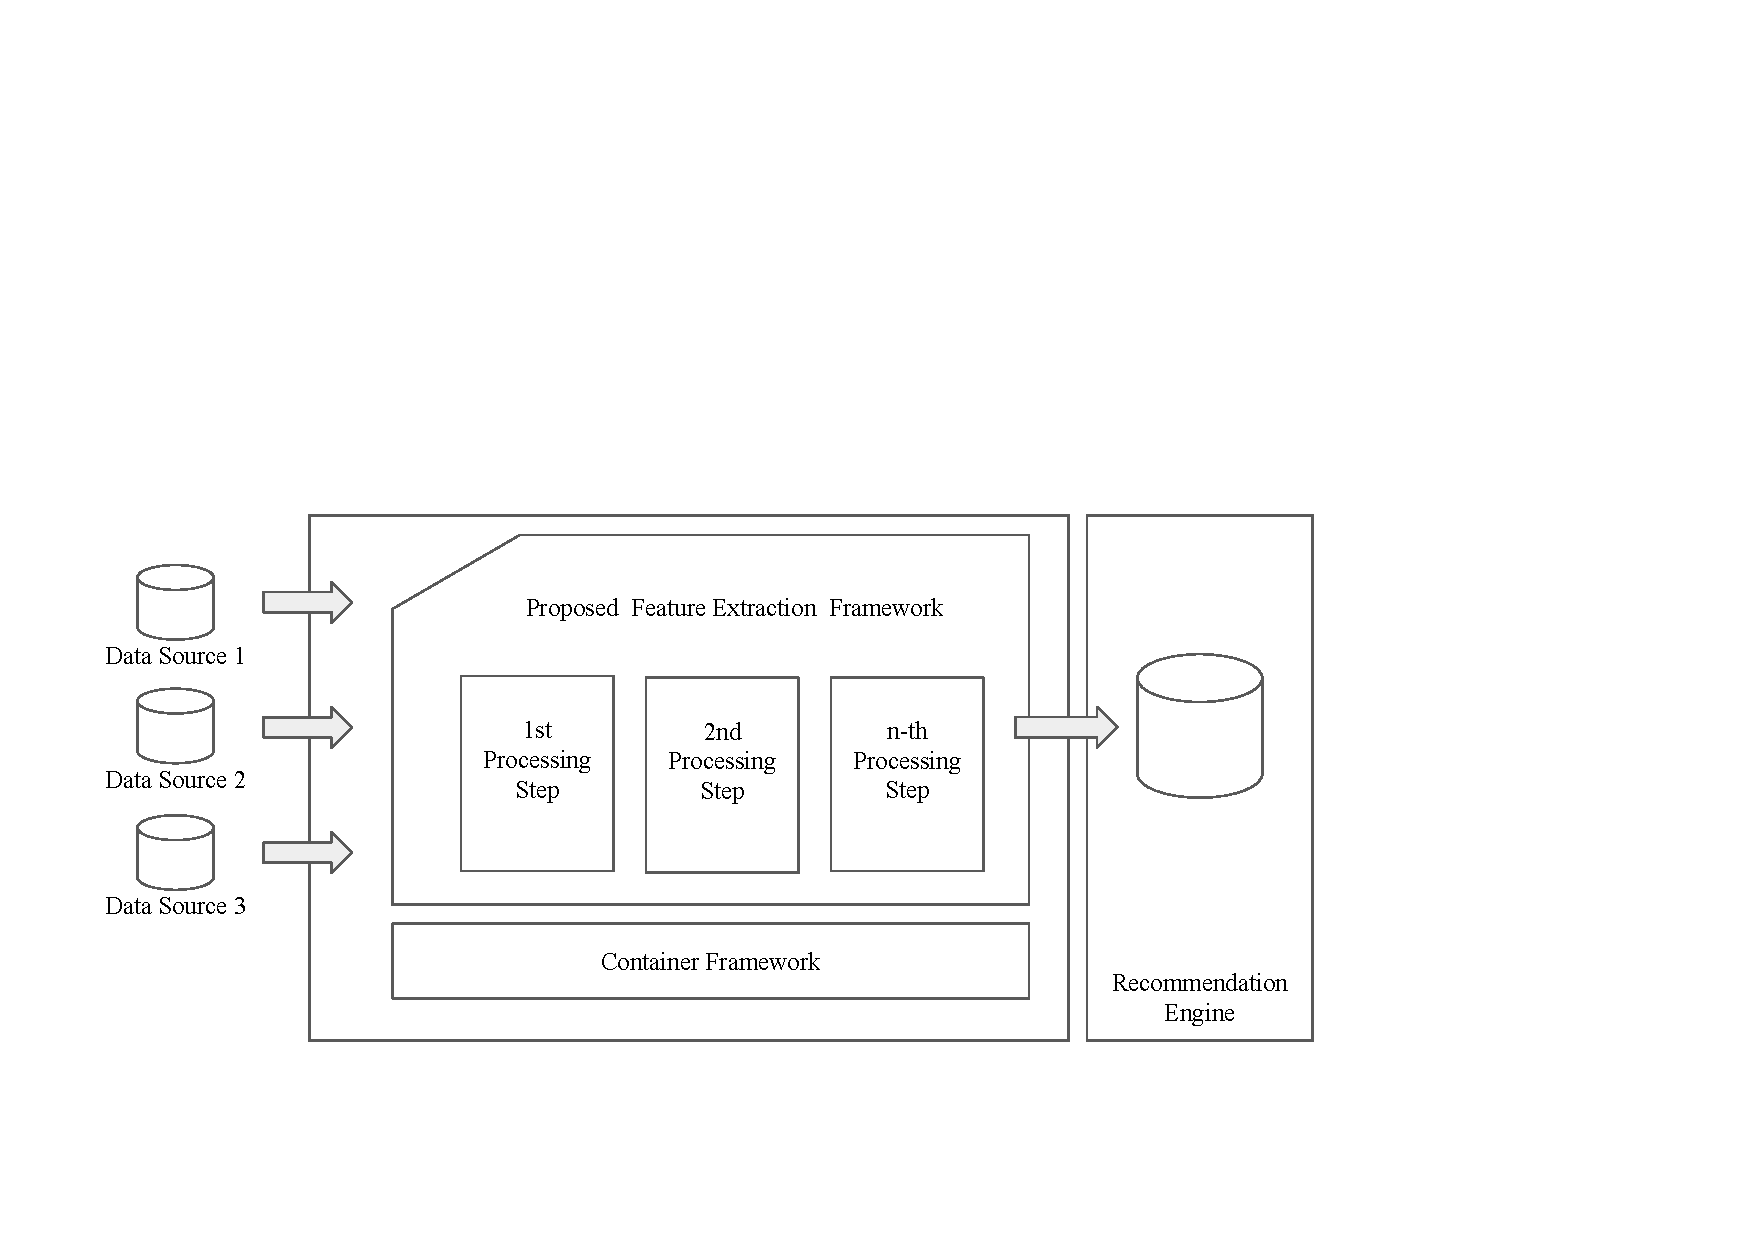
\includegraphics[width=0.9\textwidth]{concept-framework}\\
  \caption{Basic concept of feature extraction framework}
  \label{fig:basicconcept}
\end{figure}

To satisfy the requirements of a simple adaptable and highly reliable system a modularized framework concept is suggested. A pipelined approach with adaptable components characterizes the overall framework design. A later implementation of the proposed framework is desirable. Modularized software design and development ensures a level of abstraction that aims for simple update, exchange or addition of features. Single modules are implemented encapsulated and exchange data via APIs on a transportation technology. Common data structures and interfaces are shared via libraries which are simply a further module of the framework. Several software projects and frameworks contain libraries named \textit{core} or \textit{common}. For example compare modules and components, also available as libraries, of the Apache Fink framework\footnote{https://mvnrepository.com/artifact/org.apache.flink}.
\\\\
Revisiting the in chapter \ref{cha:chapter3} stated requirements leads to the breakdown of the framework into the following modules:
\begin{itemize}
\item Source adapters
\item Parsing pipeline
\item Output adapter
\item Error pipeline
\end{itemize}
In addition to handle underlying data transfer and processing a technical container framework is used. This simplifies the implementation of the feature extraction framework and abstracts the heavy lifting of data processing, data distribution and data management.
\\\\
The pipeline concept facilitates the handling of single and multiple source problems analyzed in chapter \ref{cha:chapter2}. A three step approach towards clean features is chosen to tackle structural problems and issues on entity level. Internally the framework must use a one data schema to reduce overhead on transformation as well as minimize the introduction of errors.

\section{Concept and use of the container framework \label{sec:containerframework}}

Many data processing frameworks are available nowadays. Especially the trend of big data emerged frameworks on different abstraction layers. Most of them have their foundations in widely known concept of Map Reduce\cite{dean_ghemawat_2008} or any of its descendants. Promising Open source examples in this case are among others Apache Flink\cite{flink_2017}, Apache Samza\cite{samza_2017}, Apace Spark\cite{spark_2017} or Kafak Streams\cite{kafka_2017}. From a conceptual view the container framework hides away underlying data transportation and enables the use of user defined code and user defined functions. At this place the in the previous paragraph defined modules can introduced. This abstract concept will allow to exchange the underlying container framework as well as consecutive modules. In the next chapter, chapter \ref{cha:chapter5}, after evaluation the best suitable container frameworks is determined.

\section{Concept of the input adapter \label{sec:inputadapter}}

The input adapters are mainly responsible for format and schema specific raw representation of incoming data. A raw schema does not support deterministic values but defines a set of attributes necessary for further processing steps. It is applicable for any data source publishing the respective information entity. The drawbacks of heterogeneous encoding formats is covered in section \ref{sec:stateanalysis}. From this we know it is essential to find a common and flexible way to represent data within one system. The concepts does not make any suggestions regarding the format to be chosen, as the framework must not rely on implementation specifications. It only suggests that one common encoding format for the entire framework is used to avoid translation overhead and internal error sources. For a generalization purpose the concept defines a library which enables an easy adaption to multiple data sources with their formats and schemas. Example formats can be found on the y-axis in figure \ref{fig:inputadapter}. On the x-axis the some raw entity type are displayed. For instance, if the features for \textit{Address} entities have to be found across different sources the library provides a tool set to define the input source format and the output schema. Furthermore the input adapter provides the functionality to combine a specific input source format with a specific output entity an an abstract level. This allows the aggregation of one entity type over several data sources. Compare figure \ref{fig:inputadapter}. In a concrete case the developer must be offered a interface to define a user defined function (UDF)\footnote{A UDF is a function that is executed in a bigger context, accepts parameters performs non-side-effecting transformation and returns the result.} to map between source schema and the raw target schema. 

Additional source depended knowledge can be applied in the UDF. For instance, internal quantities and units can be transformed to international standards. The concept defines a library which combines a custom source schema on a predefined (or custom) data source, mapping function to translate the source schema and the definition of the raw target schemas. The UDF has a very simple interface, as it is defined as a function mapping a custom source schema to a raw target schema. 

\begin{figure}[htb]
  \centering
  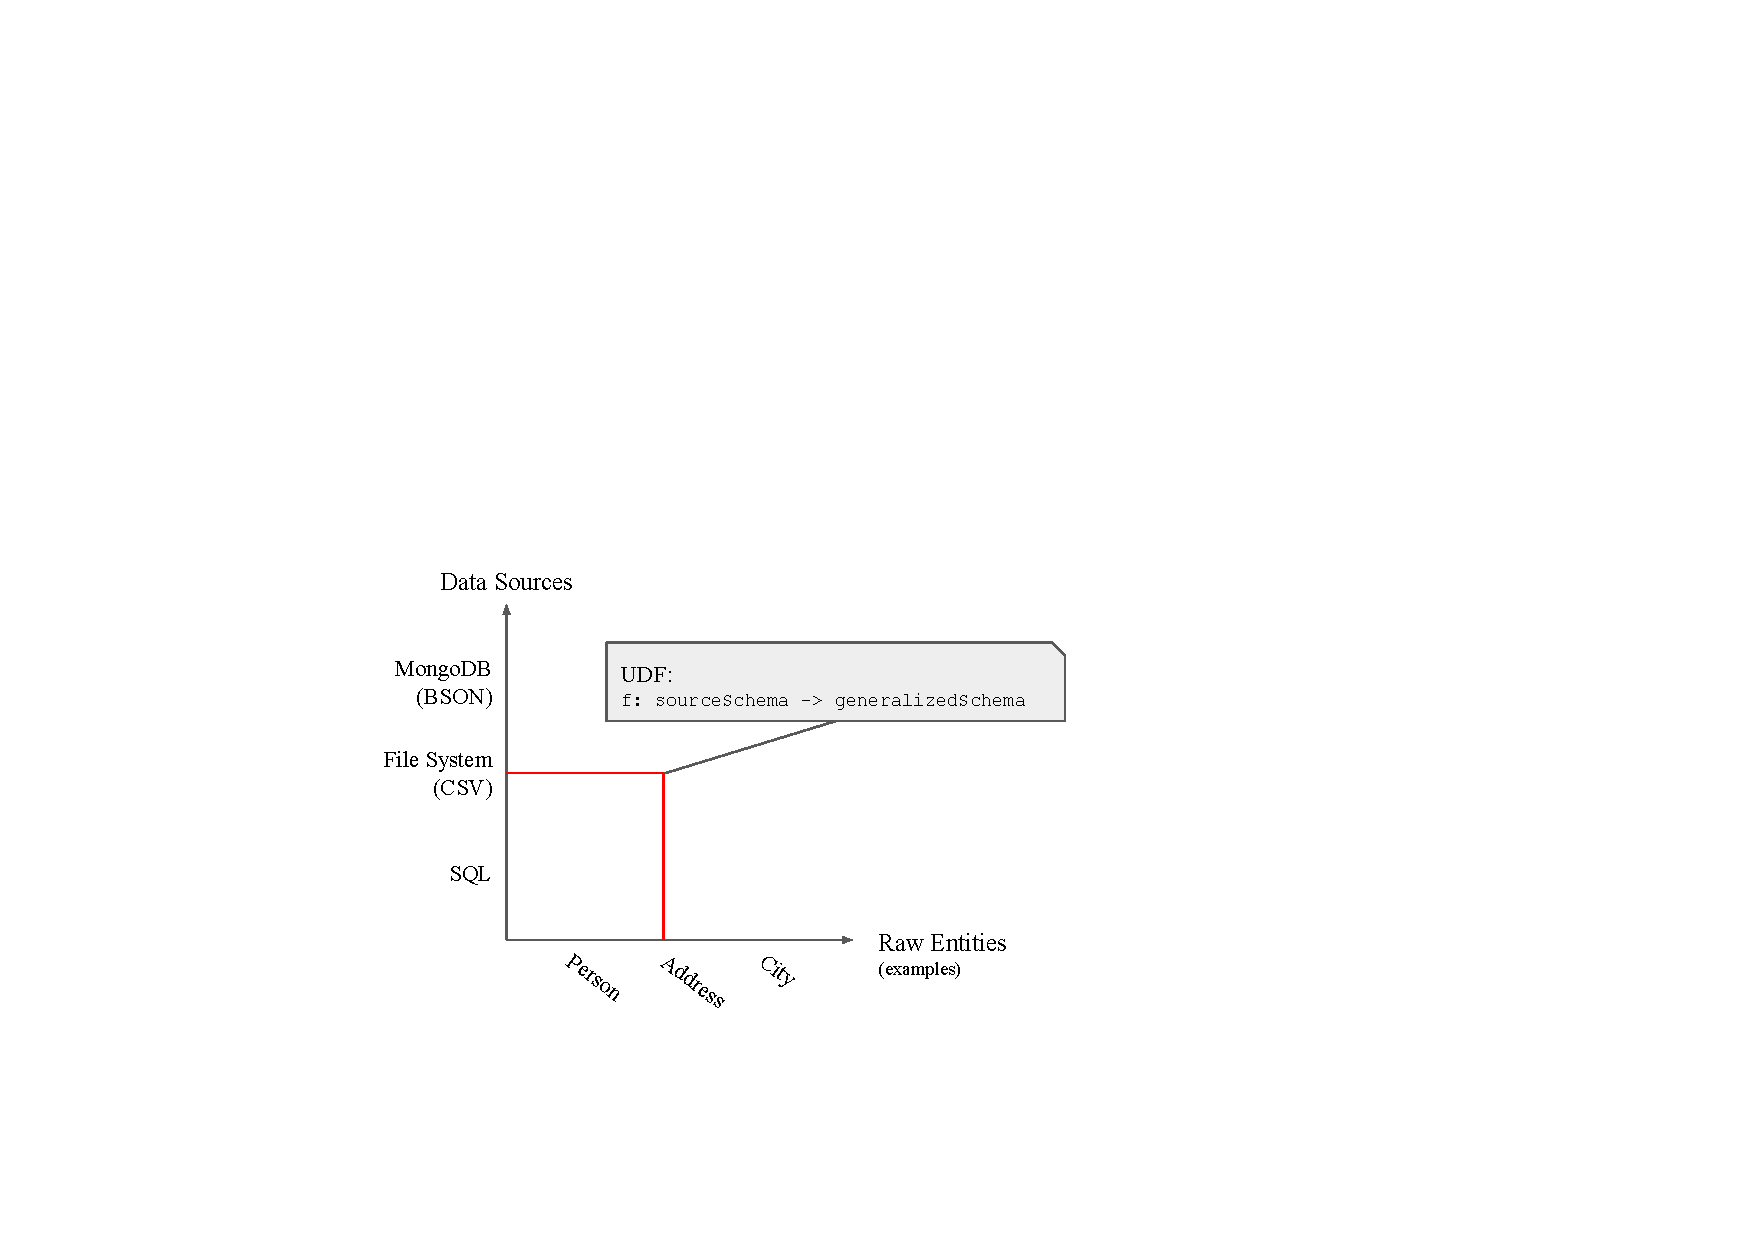
\includegraphics[width=0.6\textwidth]{input-adapter}\\
  \caption{Concept of input adapter library}
  \label{fig:inputadapter}
\end{figure}

\section{Concept of parsing pipeline\label{sec:ppln}}

The core of the processing framework is the centralized parsing pipeline. At this point a raw schema is transfered to a generalized schema. The difference here is that the raw schema can be considered as stable and therefore adequate transformation functions can be applied. It is to be provided by a developer and is defined on domain level in which the proposed framework is operating in. The concept suggests that the transformation is split up in different steps which perform different types of computations on the respective raw entity. As already explained in the previous section, section \ref{sec:inputadapter}, the concept of UDFs provides a flexible method of introducing custom functionality into a predefined system.
\\\\
Possible parsing steps among others are:
\begin{itemize}
\item Unification of different levels of normalization
\item Source independent transformation
\item Homogenization of attribute value manifestations
\end{itemize}

The abstraction of an parsing step must allow the connection to a external data repository for potential data enrichment through lookups. Another obligatory feature is a initial loading of a user defined resource such as a mapping table or a machine learning model. For this type of application asynchronous processing should be possible to avoid a blocking of the entire pipeline.

\section{Concept of pluggable output adapters\label{sec:componentsoutput}}

The pluggable output adapters are meant for further transformations of the generalized entity that results from the parsing pipeline. Based on different intents of using the homogenized data, a set of outputs is desired. From a framework aspect the output adapter is similar to the input adapters. The concept differs in a deterministic input as well as output schema or a set of deterministic output schemas, depending on the post-preparation use cases. The input schema is analog to the output schema of the parsing pipeline and due to the fact of a unified encoding format within the framework it must not produce additional development overhead. 

\section{Concept of error pipeline \label{sec:errorpipeline}}

From the requirements in section \ref{sec:error} a concept for error persistence and processing guarantees is developed. The overview in figure \ref{fig:basicconcept} show a component named Error Pipeline. The idea of the error pipeline is to create a bypass stream for faulty data. Faulty data are defined by the fact that they could not be processed in any steps of the framework. Faulty data from different steps of processing must be marked with the kind of error and the step the error occurred in. This must be done manly for a administrative purpose and manual quality check. Therefor the data can be located in different streams or data collections from where they can be fetched to analyze the underlying problem.

\section{Concept of quality assurance and ability of administration}

The quality assurance component of the automated framework is and overreaching element. The injection of of quality concerns right after parsing like manual crosschecks are facilitated. The in the error pipeline arising entities, see section \ref{sec:errorpipeline}, need a singular point of handling. Additionally the introduction of manually generalized data satisfies the need for the required processing guarantees. Those data are taken from the error pipeline and introduced into the system after manual preparation. 

Other tasks to be performed considering quality aspects are among others the control of the ongoing learning process, configuration of parsing rules and updating of mapping tables. The system needs to be defined such that on certain interaction point for all modules is available.